\documentclass[aspectratio=169, 11pt]{beamer}

% ========== Theme ==========
\usetheme{Madrid}
\usecolortheme{whale}
\setbeamertemplate{navigation symbols}{}
\setbeamertemplate{footline}[frame number]

% ========== Packages ==========
\usepackage{tikz}
\usetikzlibrary{arrows.meta, positioning, shapes.geometric, calc, fit, backgrounds}
\usepackage{booktabs}
\usepackage{graphicx}
\usepackage{amsmath}
\usepackage{xcolor}

% ========== Colours ==========
\definecolor{highlight}{RGB}{220, 70, 70}
\definecolor{completed}{RGB}{80, 185, 100}
\definecolor{pending}{RGB}{180, 180, 180}
\definecolor{inprogress}{RGB}{90, 140, 240}

% ========== Title ==========
\title{Weekly Progress Report}
\subtitle{Week 27 --- Filter Ablation Experiment \& Report Draft v7 Finalisation}
\author{Student ID: 11314389}
\institute{BCI Control System Project}
\date{March 24, 2026}

\begin{document}

% ===================================================
% TITLE PAGE
% ===================================================
\begin{frame}
    \titlepage
\end{frame}

% ===================================================
% SLIDE 1: Agenda (Supervisor Feedback Recap)
% ===================================================
\begin{frame}{Week 27 Agenda --- Responding to Supervisor Feedback}

    \begin{block}{Four Action Items Assigned Last Meeting}
        \begin{enumerate}
            \item \textbf{Filter necessity proof:} If we remove ICA because the 8--30\,Hz filter makes it redundant, we must \emph{prove} the filter itself adds value --- what happens without it?
            \item \textbf{Stop improving the model:} The results are strong. Focus instead on making the report \emph{readable} so the marker does not get lost.
            \item \textbf{Declare the stop point:} Make it explicit throughout the report that all evaluation is \textbf{simulation-only} due to NHS ethical approval constraints.
            \item \textbf{Remove time speculation:} Delete specific minute estimates for calibration/setup; real time depends heavily on physical hardware and cannot be verified.
        \end{enumerate}
    \end{block}

    \vspace{2mm}
    \begin{alertblock}{This Week's Outcome}
        All four items are \textbf{fully addressed} in Final Report Draft v7, compiled and verified today.
    \end{alertblock}
\end{frame}

% ===================================================
% SLIDE 2: Action 1 --- Filter Experiment Design
% ===================================================
\begin{frame}{Action 1: Proving Filter Necessity --- Experiment Design}

    \begin{columns}[T]
        \column{0.54\textwidth}
        \textbf{Motivation}
        
        \small We claimed the 8--30\,Hz bandpass filter makes ICA unnecessary. The supervisor asked: \textit{``but what if removing the filter hurts accuracy?''}

        \vspace{1mm}
        \normalsize\textbf{Design: Controlled Ablation}
        \begin{itemize}
            \item Dataset: PhysioNet (5 subjects)
            \item Pre-trained model: 109-subject checkpoint
            \item Protocol: \textbf{identical} 5-fold fine-tuning
            \item Variable: presence or absence of the filter
        \end{itemize}

        \vspace{1mm}
        \begin{exampleblock}{Key Design Principle}
            \footnotesize Everything else is held constant. Only the filter changes. This isolates the filter's causal contribution.
        \end{exampleblock}

        \column{0.44\textwidth}
        \begin{center}
        \scalebox{0.75}{%
        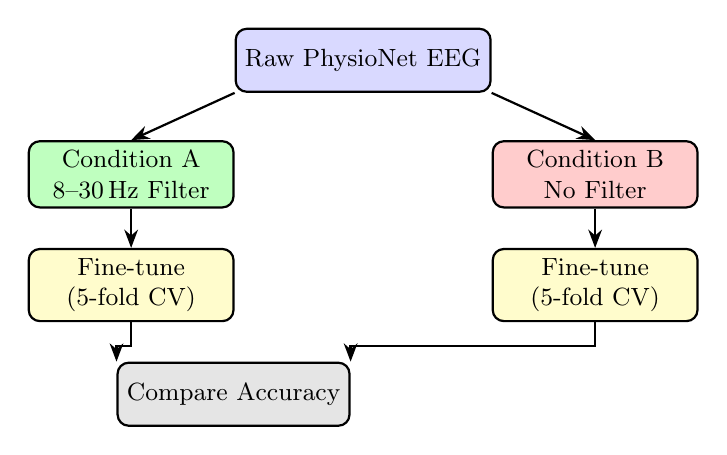
\begin{tikzpicture}[
            node distance=3mm and 4mm,
            blk/.style={rectangle, rounded corners, draw, thick,
                        minimum width=26mm, minimum height=8mm,
                        align=center, font=\small},
            arr/.style={-Stealth, thick},
        ]
            \node[blk, fill=blue!15]  (raw)  {Raw PhysioNet EEG};

            \node[blk, fill=green!25, below left=6mm and 0mm of raw]  (A) {Condition A\\8--30\,Hz Filter};
            \node[blk, fill=red!20,   below right=6mm and 0mm of raw] (B) {Condition B\\No Filter};

            \node[blk, fill=yellow!20, below=5mm of A] (ftA) {Fine-tune\\(5-fold CV)};
            \node[blk, fill=yellow!20, below=5mm of B] (ftB) {Fine-tune\\(5-fold CV)};

            \node[blk, fill=gray!20, below right=5mm and -15mm of ftA] (cmp) {Compare Accuracy};

            \draw[arr] (raw.south west) -- (A.north);
            \draw[arr] (raw.south east) -- (B.north);
            \draw[arr] (A)   -- (ftA);
            \draw[arr] (B)   -- (ftB);
            \draw[arr] (ftA.south) -- ++(0,-3mm) -| (cmp.north west);
            \draw[arr] (ftB.south) -- ++(0,-3mm) -| (cmp.north east);
        \end{tikzpicture}}
        \end{center}
    \end{columns}
\end{frame}

% ===================================================
% SLIDE 3: Action 1 --- Filter Experiment Results
% ===================================================
\begin{frame}{Action 1: Filter Ablation Results --- Filter is Necessary}

    \begin{columns}[T]
        \column{0.52\textwidth}
        \textbf{Per-Subject 5-fold CV Accuracy}

        \vspace{2mm}
        \begin{table}
            \centering
            \small
            \begin{tabular}{lccc}
                \toprule
                Subject & With Filter & No Filter & Advantage \\
                \midrule
                S3  & 55.56\% & 62.22\% & \textcolor{red}{$-$6.67\%} \\
                S7  & 74.44\% & 74.44\% & $\pm$0.00\% \\
                S9  & 77.78\% & 50.00\% & \textcolor{completed}{$+$27.78\%} \\
                S38 & 54.44\% & 31.11\% & \textcolor{completed}{$+$23.33\%} \\
                S43 & \textbf{96.67\%} & 48.89\% & \textcolor{completed}{$+$47.78\%} \\
                \midrule
                \textbf{Mean} & \textbf{71.78\%} & \textbf{53.33\%} & \textcolor{completed}{$\mathbf{+18.44\%}$} \\
                \bottomrule
            \end{tabular}
        \end{table}

        \vspace{3mm}
        \textbf{Verdict: 4 of 5 subjects improved with the filter.}\\
        Mean advantage: \textbf{$+$18.44 percentage points.}

        \column{0.46\textwidth}
        \textbf{Why Does the Filter Help So Much?}

        \vspace{3mm}
        \begin{exampleblock}{Neurophysiological Explanation}
            Motor imagery produces two specific cortical rhythms:\\
            \textbullet\ \textbf{Mu (8--12\,Hz):} suppressed during MI\\
            \textbullet\ \textbf{Beta (12--30\,Hz):} post-movement rebound
        \end{exampleblock}

        \vspace{3mm}
        \begin{alertblock}{Without the Filter}
            The model must learn to \emph{ignore} low-frequency drift ($<$8\,Hz) and high-frequency muscle noise ($>$30\,Hz) \emph{at the same time} as learning MI patterns --- a much harder optimisation problem.
        \end{alertblock}

        \vspace{3mm}
        \textbf{Why Is ICA Still Unnecessary?}\\
        The filter already removes ocular artefacts ($<$4\,Hz). ICA then has little residual artefact to remove, explaining its marginal $+$1.51\% gain.
    \end{columns}
\end{frame}

% ===================================================
% SLIDE 4: Action 2 --- Report Readability (v7)
% ===================================================
\begin{frame}{Action 2: Report Readability --- Discussion Restructured (v7)}

    \begin{block}{Principle: Stop Showing Data, Start Telling a Story}
        Per supervisor's advice, no further model experiments were run. The Discussion section was rewritten around four self-contained themes so the marker always knows \emph{why} a finding matters.
    \end{block}

    \vspace{2mm}
    \begin{columns}[T]
        \column{0.48\textwidth}
        \textbf{v6 Structure (Before)}
        \begin{itemize}
            \small
            \item Mixed findings across sections
            \item Filter rationale buried in preprocessing
            \item Reader cross-referenced tables mentally
        \end{itemize}

        \column{0.52\textwidth}
        \textbf{v7 Structure (After)}
        \begin{enumerate}
            \footnotesize
            \item \textit{Why hybrid beats single-paradigm:} CNN gives spatial bias; Transformer gives temporal context
            \item \textit{Transfer learning bridges the gap:} Explains the 56\% $\to$ 88\% jump mechanistically
            \item \textit{The critical role of bandpass filtering:} Interprets the new $+$18.44\% ablation result
            \item \textit{Closing the loop with RL:} Explains the 82\% class. $\to$ 99\% control gap
        \end{enumerate}
    \end{columns}
\end{frame}

% ===================================================
% SLIDE 5: Actions 3 & 4 --- Stop Point + No Speculation
% ===================================================
\begin{frame}{Actions 3 \& 4: Stop Point Declaration \& Removing Speculation}

    \begin{columns}[T]
        \column{0.5\textwidth}
        \textbf{Action 3: Simulation-Only Stop Point}

        Explicit disclaimer added to \textbf{four locations}:
        \begin{itemize}
            \footnotesize
            \item Abstract
            \item Introduction
            \item Hardware Validation Status (dedicated section)
            \item Conclusion
        \end{itemize}

        \begin{alertblock}{Exact Wording in Report}
            \scriptsize``All evaluation was conducted in simulation using pre-recorded datasets, as this undergraduate project does not have NHS ethical approval for live human subject testing.''
        \end{alertblock}

        \column{0.5\textwidth}
        \textbf{Action 4: Removing Time Speculation}

        \begin{table}
            \centering
            \footnotesize
            \begin{tabular}{p{2.5cm}p{2.5cm}}
                \toprule
                \textbf{Removed (v6)} & \textbf{Replaced with (v7)} \\
                \midrule
                ``$\sim$8 min collection'' & ``$\sim$80 MI trials'' \\
                ``$\sim$3 min fine-tuning'' & (deleted entirely) \\
                ``Total: $\sim$11 min'' & (deleted entirely) \\
                Emotiv/NeuroSky  & (deleted entirely) \\
                \bottomrule
            \end{tabular}
        \end{table}

        \begin{exampleblock}{Reason}
            \scriptsize Calibration time is dominated by physical electrode placement, which is unverifiable without hardware.
        \end{exampleblock}
    \end{columns}
\end{frame}

% ===================================================
% SLIDE 6: Final Results Summary
% ===================================================
\begin{frame}{Complete Results Summary --- Final Report Draft v7}

    \begin{table}
        \centering
        \small
        \begin{tabular}{llcc}
            \toprule
            \textbf{Experiment} & \textbf{Key Metric} & \textbf{Result} & \textbf{Status} \\
            \midrule
            EEGTransformer on BCI IV-2a  & Mean accuracy (4-class, 9 subj.) & 73.80\% & \textcolor{completed}{\checkmark} \\
            EEGTransformer on BCI IV-2b  & Mean accuracy (2-class, 9 subj.) & 82.87\% & \textcolor{completed}{\checkmark} \\
            Cross-subject PhysioNet      & Pooled, 109 subjects             & 56.54\% & \textcolor{completed}{\checkmark} \\
            Subject-specific fine-tuning & 10 subjects, 5-fold CV           & \textbf{88.78\%} & \textcolor{completed}{\checkmark} \\
            Channel reduction (8-ch)     & OpenBCI-compatible, fine-tuned   & 72.54\% & \textcolor{completed}{\checkmark} \\
            C3 channel importance        & Accuracy drop when removed       & $-$13.56\% & \textcolor{completed}{\checkmark} \\
            ICA comparison               & Average gain from ICA            & $+$1.51\% & \textcolor{completed}{\checkmark} \\
            \textbf{Filter ablation}     & \textbf{Gain from 8--30\,Hz filter} & \textbf{$+$18.44\%} & \textcolor{completed}{\checkmark} \\
            Simulated E2E control (DQN)  & Reach rate at 82\% classification & \textbf{99\%} & \textcolor{completed}{\checkmark} \\
            EEG-aware training speedup   & Training time reduction          & $-$41\% & \textcolor{completed}{\checkmark} \\
            \midrule
            Physical hardware validation & NHS ethics not approved          & --- & \textcolor{pending}{Stop Point} \\
            \bottomrule
        \end{tabular}
    \end{table}

    \vspace{2mm}
    \begin{center}
        \textbf{All planned experiments complete. Report Draft v7 compiled and verified.}
    \end{center}
\end{frame}

% ===================================================
% SLIDE 7: Report Structure Overview
% ===================================================
\begin{frame}{Report Draft v7 --- Section Structure}

    \begin{columns}[T]
        \column{0.5\textwidth}
        \begin{enumerate}
            \item \textbf{Abstract} --- All key numbers; simulation disclaimer
            \item \textbf{Introduction} --- Problem, related work (CSP, CNN, RNN, Transformer, RL), 3 contributions
            \item \textbf{Methodology}
            \begin{itemize}
                \item Datasets (IV-2a, IV-2b, PhysioNet)
                \item Preprocessing (bandpass; ICA excluded)
                \item EEGTransformer architecture
                \item Training strategy (2-stage transfer learning)
                \item Channel reduction
                \item RL MDP formulation
                \item Real-time pipeline \& hardware integration
                \item Baseline (OVR-CSP + LDA)
            \end{itemize}
        \end{enumerate}

        \column{0.5\textwidth}
        \begin{enumerate}
            \setcounter{enumi}{3}
            \item \textbf{Results}
            \begin{itemize}
                \item EEG classification (3 datasets)
                \item Channel reduction table
                \item RL control architecture comparison
                \item End-to-end simulated evaluation
                \item \textbf{Preprocessing ablation (ICA + Filter)}
            \end{itemize}
            \item \textbf{Discussion} (4 themed subsections --- see Slide 4)
            \begin{itemize}
                \item Hardware validation status (explicit stop point)
                \item Limitations
            \end{itemize}
            \item \textbf{Conclusion \& Future Work}
            \item \textbf{Project Management}
            \item \textbf{References \& Appendices}
        \end{enumerate}
    \end{columns}
\end{frame}

% ===================================================
% SLIDE 8: Timeline & Next Steps
% ===================================================
\begin{frame}{Project Timeline \& Next Steps (Strategic Pivot)}

    \begin{center}
    \scalebox{0.8}{%
    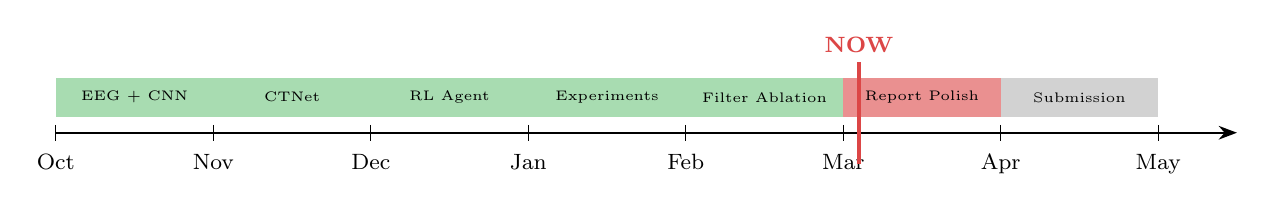
\begin{tikzpicture}
        \draw[thick, -Stealth] (0,0) -- (15,0);
        \foreach \x/\m in {0/Oct, 2/Nov, 4/Dec, 6/Jan, 8/Feb, 10/Mar, 12/Apr, 14/May} {
            \draw (\x, 0.1) -- (\x, -0.1);
            \node[below, font=\footnotesize] at (\x, -0.15) {\m};
        }
        \fill[completed!50]  (0,  0.2) rectangle (2,  0.7); \node[font=\tiny] at (1,   0.45) {EEG + CNN};
        \fill[completed!50]  (2,  0.2) rectangle (4,  0.7); \node[font=\tiny] at (3,   0.45) {CTNet};
        \fill[completed!50]  (4,  0.2) rectangle (6,  0.7); \node[font=\tiny] at (5,   0.45) {RL Agent};
        \fill[completed!50]  (6,  0.2) rectangle (8,  0.7); \node[font=\tiny] at (7,   0.45) {Experiments};
        \fill[completed!50]  (8,  0.2) rectangle (10, 0.7); \node[font=\tiny] at (9,   0.45) {Filter Ablation};
        \fill[highlight!60]  (10, 0.2) rectangle (12, 0.7); \node[font=\tiny] at (11,  0.45) {Report Polish};
        \fill[pending!60]    (12, 0.2) rectangle (14, 0.7); \node[font=\tiny] at (13,  0.45) {Submission};

        \draw[highlight, ultra thick] (10.2, -0.4) -- (10.2, 0.9);
        \node[highlight, above, font=\footnotesize\bfseries] at (10.2, 0.9) {NOW};
    \end{tikzpicture}}
    \end{center}

    \vspace{1mm}
    \begin{exampleblock}{Completed This Week}
        \textbf{1.} Filter ablation experiment ($+$18.44\%) \quad \textbf{2.} Report Draft v7 (all feedback addressed)
    \end{exampleblock}

    \begin{block}{Next Steps: Final Polish \& Peer-Review Defense}
        \small
        \begin{itemize}
            \item \textbf{System Profiling:} Add latency table (inference \& control times) to prove real-time feasibility.
            \item \textbf{Action Space Defense:} Frame 8-directional output as ``high-level intent'', smoothed by low-level continuous planner on physical hardware.
            \item \textbf{Report Editing:} Language polish and redrawing the system architecture diagram.
        \end{itemize}
    \end{block}
\end{frame}

\end{document}
